\documentclass[12pt]{article}
\usepackage[english]{babel}
\usepackage[utf8x]{inputenc}
\usepackage{amsmath}
\usepackage{tikz}
\usetikzlibrary{arrows,automata}
\begin{document}

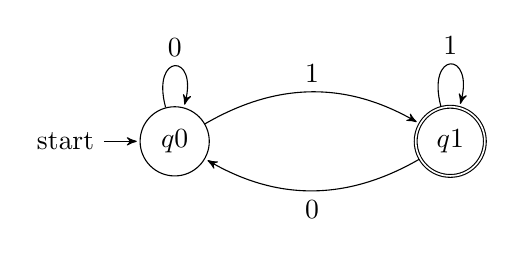
\begin{tikzpicture}[->,>=stealth',shorten >=1pt,auto,node distance=3.5cm,scale = 1,transform shape]
\node[state,initial] (q0) {$q0$};
\node[state,accepting] [right of=q0](q1) {$q1$};
\path (q0)	edge	[loop above]	node{$0$} (q0)
(q0)	edge	[bend left]	node{$1$} (q1)
(q1)	edge	[bend left]	node{$0$} (q0)
(q1)	edge	[loop above]	node{$1$} (q1)
;\end{tikzpicture}

\end{document}